\subsubsection{嵌入式存储器}
片上存储器由功能固定的 MPU，可配置的 MPU 和 MMU 管理：
\begin{table}[H]
    \centering
    \caption{片上存储器的 MPU 和 MMU 结构}
    \label{table:MPU_MMU_for_Internal_Memory}
    \begin{tabular}[h]{ |p{4cm}|p{2cm}|p{3cm}|p{3cm}|p{3cm}|}
        \hline
        \rowcolor{lightgray}
        & & \multicolumn{2}{c|}{地址范围} &  \\
        \cline{2-5}
        \rowcolor{lightgray}
        \multirow{-2}*{存储器名字} & \multirow{-2}*{大小} & 开始 & 结束 & \multirow{-2}*{管理存储器的 MPU} \\
        \hline
        ROM0 & 384 KB & 0x4000\_0000 & 0x4005\_FFFF &  Static MPU \\ \hline
		ROM1 & 64 KB & 0x3FF9\_0000 & 0x3FF9\_FFFF & Static MPU \\ \hline
		\multirow{2}{*}{SRAM0} & 64 KB & 0x4007\_0000 & 0x4007\_FFFF & Static MPU \\ 
		 & 128 KB & 0x4008\_0000 & 0x4009\_FFFF & SRAM0 MMU \\ \hline
		\multirow{3}{*}{SRAM1 (多地址访问)} & 128 KB & 0x3FFE\_0000 & 0x3FFF\_FFFF & Static MPU \\
		 & 128 KB & 0x400A\_0000 & 0x400B\_FFFF & Static MPU \\
		 & 32 KB & 0x4000\_0000 & 0x4000\_7FFF & Static MPU \\ \hline
		\multirow{2}{*}{SRAM2} & 72 KB & 0x3FFA\_E000 & 0x3FFB\_FFFF & Static MPU \\
		 & 128 KB & 0x3FFC\_0000 & 0x3FFD\_FFFF & SRAM2 MMU \\ \hline
		\multirow{2}{*}{RTC FAST (多地址访问)} & 8 KB & 0x3FF8\_0000 & 0x3FF8\_1FFF & RTC FAST MPU \\
		 & 8 KB & 0x400C\_0000 & 0x400C\_1FFF & RTC FAST MPU \\ \hline
		RTC SLOW & 8 KB & 0x5000\_0000 & 0x5000\_1FFF & RTC SLOW MPU \\ \hline
    \end{tabular}
\end{table}


\subparagraph{Static MPU}
ROM0，ROM1，SRAM0 的低 64 KB，SRAM1 和 SRAM2 的低 72 KB 由 Static MPU 控制。 这些 MPU 由硬件控制，不能由软件配置。 它们仅通过当前进程的 PID  管理进程对存储器区域的访问。当进程的 PID 为 0 或 1 时，可以使用表 \ref{table:MPU_MMU_for_Internal_Memory} 中指定的地址段读取（当存储器为 RAM 时用相应地址段写入）存储器。当 PID 为 2 到 7，存储器不可被访问。

\subparagraph{RTC FAST \& RTC SLOW MPU}
8 KB 的 RTC FAST Memory 以及 8 KB 的 RTC SLOW Memory 由两个可配置的 MPU 控制。通过配置 
RTC\_CNTL\_ RTC\_PID\_CONFIG\_REG 和 DPORT\_AHBLITE\_MPU\_TABLE\_RTC\_REG 寄存器，MPU 可以允许或禁止每个单独的 PID 访问存储器。通过设置这些寄存器中某个位，可以允许相应的 PID 从存储器读取或写入数据，清除该位则禁止相应的 PID 从存储器读取或写入数据。PID 为 0 和 1 的进程始终可以访问 RTC SLOW 存储器，该配置无法修改。表 \ref{table:MPU_for_RTC_FAST_Memory} 和 \ref{table:MPU_for_RTC_SLOW_Memory} 描述了寄存器位与 PID 之间的映射关系。


\begin{table}[H]
    \centering
    \caption{管理 RTC FAST Memory 的 MPU}
    \label{table:MPU_for_RTC_FAST_Memory}
   
     \begin{tabular}[h]{ |p{2cm}|p{3cm}|p{3cm}|p{7cm}|}
        \hline
        \rowcolor{lightgray}
        & \multicolumn{2}{c|}{边界地址} & 权限 \\
        \cline{2-4}
        \rowcolor{lightgray}
        \multirow{-2}*{大小} & 低 & 高 & \makecell{PID\\RTC\_CNTL\_RTC\_PID\_CONFIG 位} \\
        \hline
        8 KB & 0x3FF8\_0000 & 0x3FF8\_1FFF & \multirow{2}*{\makecell{0 1 2 3 4 5 6 7\\0 1 2 3 4 5 6 7}} \\
        \cline{1-3}
        8 KB & 0x400C\_0000 & 0x400C\_1FFF & \\
        \hline
    \end{tabular}
\end{table}


\begin{table}[H]
    \centering
    \caption{管理 RTC SLOW Memory 的 MPU}
    \label{table:MPU_for_RTC_SLOW_Memory}
    
     \begin{tabular}[h]{ |p{1cm}|p{2cm}|p{2cm}|p{2cm}|p{7.5cm}|}
    
        \hline
        \rowcolor{lightgray}
        & \multicolumn{2}{c|}{边界地址} & \multicolumn{2}{c|}{权限} \\
        \cline{2-5}
        \rowcolor{lightgray}
        \multirow{-2}*{大小} & 低 & 高 & PID = 0/1 & \makecell{PID\\DPORT\_AHBLITE\_MPU\_TABLE\_RTC\_REG 位} \\
        \hline
        8 KB & 0x5000\_0000 & 0x5000\_1FFF & 读/写 & \makecell{2 3 4 5 6 7\\0 1 2 3 4 5} \\
        \hline
    \end{tabular}
\end{table}


寄存器 RTC\_CNTL\_RTC\_PID\_CONFIG\_REG 是 RTC 外设的一部分，只能由 PID 为 0 的进程修改; 寄存器 DPORT \_AHBLITE\_MPU\_TABLE\_RTC\_REG 是一个 Dport 寄存器，可以由 PID 为 0 或 1 的进程修改。

\subparagraph{管理 SRAM0 和 SRAM2 高 128 KB 的 MMU}

SRAM0 的高 128 KB 和 SRAM 的 高 128 KB 都由 MMU 管理。这些 MMU 不仅可以和 MPU 一样允许或禁止进程访问它们管理的存储器范围，而且还能够将 CPU 读取或写入的地址（虚地址）转换到存储器中可能不同的地址（实地址）。

为了实现这一点，片上 RAM MMU 将其管理的存储器范围划分为 16 页。 页大小可配置为 8 KB，4 KB 和 2 KB。 当页大小为 8 KB 时，16 页包含了整个 128 KB 的存储器空间; 当页大小为 4 KB 或 2 KB 时，存储器空间的末端将有分别为 64 KB 或 96 KB 区域不受 MPU 管理。 类似于虚地址和实地址，页也可分为虚地址页和实地址页两种：MMU 可以将虚地址页内的地址转换为实地址页内的地址。

对于 PID 为 0 和 1 的进程，虚地址页与实地址页的地址映射是一对一的。即对某个虚地址页的读取或写入总被转换为对完全相同的实地址页的读取或写入。这允许在 PID 0 和/或 1 下运行的操作系统总是能够访问整个物理存储器范围。

但是对于 PID 为 2 到 7 的进程，MMU 可以基于每个 PID，重新配置每个虚地址页，使其映射到不同的实地址页。因此，对虚地址页内的偏移量的读取和写入可被转换为对不同实地址页内的相同偏移量的读取和写入。如图 \ref{Figure:MMU_example} 所示，CPU（运行 PID 为 2 到 7 的进程）尝试访问存储器地址 0x3FFC\_2345。该地址在虚地址页 1 的存储器区域内，偏移量为 0x0345。MMU 被指示将该 PID 的进程对虚地址页 1 的访问转换为实地址页 2 的访问。因此，存储器访问被重新定向为访问虚拟地址页 2 中相同的偏移，实际访问的实地址为 0x3FFC\_\textbf{4}345。以下示例中的页大小为 8 KB。

\begin{figure}[h!]
    \centering
    \fbox{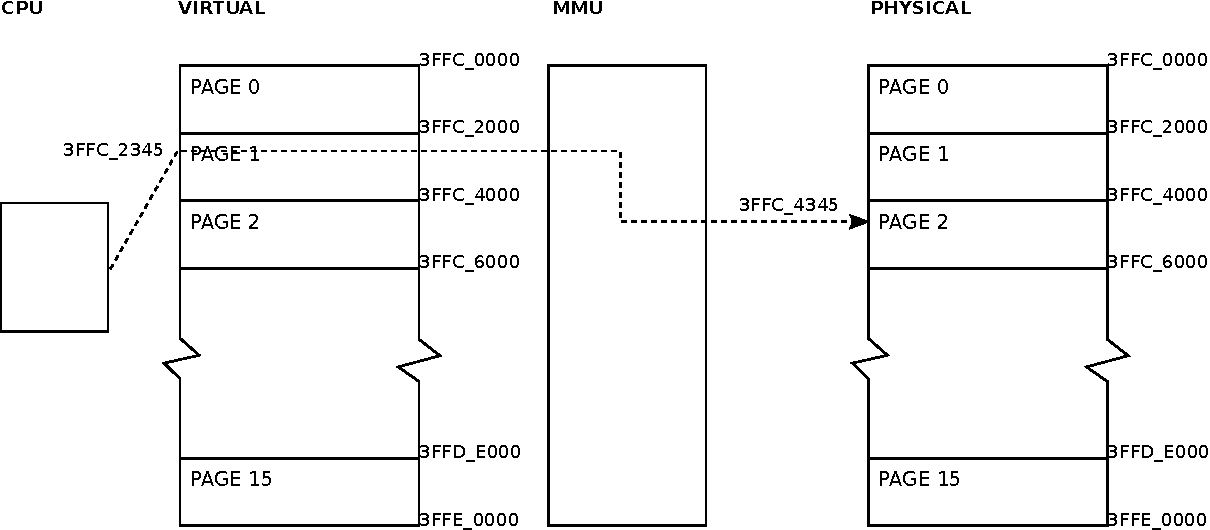
\includegraphics[width=0.9\textwidth]{./04-MMUMPU/figures/mmu_example.pdf}}
    \caption{MMU 访问示例}
    \label{Figure:MMU_example}
\end{figure}


\begin{table}[H]
    \centering
    \caption{管理片上 SRAM 0 和 SRAM2 剩余 128 KB 的 MMU 页模式}
    \label{table:Page_Mode_of_MMU_for_remaining_128KB_of_Internal_SRAM_0_2}
   
    
    \begin{tabular}[h]{ |p{6cm}|p{6cm}|p{3cm}|} 
    
        \hline
        \rowcolor{lightgray}
        DPORT\_IMMU\_PAGE\_MODE & DPORT\_DMMU\_PAGE\_MODE & 页大小 \\
        \hline
        0 & 0 & 8 KB \\
        \hline
        1 & 1 & 4 KB \\
        \hline
        2 & 2 & 2 KB \\
        \hline
    \end{tabular}
\end{table}

\subparagraph{非 MMU 管理的存储器}
对于 MMU 管理的 SRAM0 和 SRAM2 区域，页大小可配置为 8 KB，4 KB 和 2 KB。如表 \ref{table:Page_Mode_of_MMU_for_remaining_128KB_of_Internal_SRAM_0_2} 所示，页大小通过寄存器 DPORT\_IMMU\_PAGE\_MODE\_REG 和 DPORT\_DMMU\_PAGE\_MODE\_REG 中的 DPORT\_IMMU\_PAGE\_MODE (对于 SRAM0) 和 DPORT\_DMMU\_PAGE\_MODE (对于 SRAM2) 位设置。
因为每个存储器区域的页数量固定为 16，所以当页大小为 8 KB 时，这 16 页覆盖的存储器空间为 128 KB；当页大小为 4 KB 时，覆盖的存储器空间为 64 KB；当页大小为 2 KB 时，覆盖的存储器空间为 32 KB。

因此，对于 8 KB 页，整个存储器由 MMU 管理；但对于其它页大小，存储器的 128 KB 有一部分不受 MMU 管理。具体是，对于 4 KB 的页大小，不受 MMU 管理的区域是 0x4009\_0000 到 0x4009\_FFFF 和 0x3FFD\_0000 到 0x3FFD\_FFFF；对于 2 KB 的页大小，不受 MMU 管理的区域是 0x4008\_8000 到 0x4009\_FFFF 和 0x3FFC\_8000 到 0x3FFD\_FFFF。这些范围可由 PID 为 0 或 1 的进程读写；PID 为 2 到 7 的进程无法访问此存储器。
 
存储器空间中，页的布局是线性的，即，MMU 管理的 SRAM0 页 \textcolor{red}{\it{n}} 覆盖的地址范围为 $0x40080000+(pagesize×\textcolor{red}{\it{n}})$ 到 $0x40080000+(pagesize×(\textcolor{red}{\it{n}}+1)-1)$；同理，MMU 管理的 SRAM2 页 \textcolor{red}{\it{n}} 覆盖的地址范围为 $0x3FFC0000+(pagesize×\textcolor{red}{\it{n}})$ 到 $0x3FFC0000+(pagesize×(\textcolor{red}{\it{n}}+1)-1)$。表 \ref{table:Page_Boundaries_SRAM0_MMU} 和 \ref{table:Page_Boundaries_SRAM2_MMU} 描述了不同页大小模式下，由 MMU 管理的 SRAM0 和 SRAM2 所有页地址范围。

\input{./04-MMUMPU/tables/Page_Boundaries_MMU_SRAM0_SRAM2_cn.tex}

\subparagraph{MMU 映射}

SRAM0 MMU 和 SRAM2 MMU，通过一组 16 个寄存器控制访问权限和虚地址页到实地址页的映射。与其它大多数 MMU 不同的是，每个寄存器控制一个\textbf{实地址}页，而不是一个虚地址页。这些寄存器决定哪些 PID 的进程 可以访问物理存储器以及哪个虚地址页映射到该寄存器控制的实地址页。表 \ref{table:DPORT_DMMU_IMMU_TABLEn_REG} 描述了这些寄存器的位。需要注意的是，这些寄存器只控制 PID 为 2 到 7 的进程的访问权限；PID 为 0 或 1 的进程总是可以读写所有的页，并且没有虚地址到实地址的映射。即无论这些寄存器的设置如何，当 PID 为 0 或 1 的进程访问页 \textcolor{red}{\it{x}} 时，总是访问实地址页 \textcolor{red}{\it{x}}。这 16 个寄存器和控制页大小的寄存器 DPORT\_IMMU\_PAGE\_MODE\_REG 和 DPORT\_DMMU\_PAGE\_MODE\_REG 只能由 PID 为 0 或 1的进程写入。

\begin{table}[H]
    \centering
    \caption{DPORT\_DMMU\_TABLE\textcolor{red}{\it{n}}\_REG 和 DPORT\_IMMU\_TABLE\textcolor{red}{\it{n}}\_REG}
    \label{table:DPORT_DMMU_IMMU_TABLEn_REG}
    \begin{tabular}[t]{|p{1cm}|p{6cm}|}
     
        \hline
        \rowcolor{lightgray}
        \verb+[+6:4\verb+]+ & PID 2\verb+~+ 7 的访问权限\\
        \hline
        0 & PID 2 \verb+~+ 7 的进程都没有访问权限。 \\
        \hline
        1 & PID 2 \verb+~+ 7 的进程都有访问权限。 \\
        \hline
        2 & 只有 PID 2 的进程有访问权限。 \\
        \hline
        3 & 只有 PID 3 的进程有访问权限。 \\
        \hline
        4 & 只有 PID 4 的进程有访问权限。 \\
        \hline
        5 & 只有 PID 5 的进程有访问权限。 \\
        \hline
        6 & 只有 PID 6 的进程有访问权限。 \\
        \hline
        7 & 只有 PID 7 的进程有访问权限。 \\
        \hline
    \end{tabular}
    \begin{tabular}[t]{|p{1cm}|p{5cm}|}
        \hline
        \rowcolor{lightgray}
        \verb+[+3:0\verb+]+ & 地址权限 \\
        \hline
        0x00 & 虚拟页 0 可访问该物理页。 \\
        \hline
        0x01 & 虚拟页 1 可访问该物理页。 \\
        \hline
        0x02 & 虚拟页 2 可访问该物理页。 \\
        \hline
        0x03 & 虚拟页 3 可访问该物理页。\\
        \hline
        0x04 & 虚拟页 4 可访问该物理页。 \\
        \hline
        0x05 & 虚拟页 5 可访问该物理页。 \\
        \hline
        0x06 & 虚拟页 6 可访问该物理页。 \\
        \hline
        0x07 & 虚拟页 7 可访问该物理页。\\
        \hline
        0x08 & 虚拟页 8 可访问该物理页。\\
        \hline
        0x09 & 虚拟页 9 可访问该物理页。 \\
        \hline
        0x10 & 虚拟页 10 可访问该物理页。 \\
        \hline
        0x11 & 虚拟页 11 可访问该物理页。\\
        \hline
        0x12 & 虚拟页 12 可访问该物理页。 \\
        \hline
        0x13 & 虚拟页 13 可访问该物理页。 \\
        \hline
        0x14 & 虚拟页 14 可访问该物理页。 \\
        \hline
        0x15 & 虚拟页 15 可访问该物理页。 \\
        \hline
    \end{tabular}
\end{table}



\subparagraph{SRAM0 和 SRAM2 MMU 的差异}

由 SRAM0 MMU 管理的存储器通过处理器指令总线被访问，而处理器通过数据总线访问由 SRAM2 MMU 控制的存储器。 因此，通常的做法是将代码存储在 SRAM0 的 MMU 页中，将数据存在 SRAM2 的 MMU 页中。 因为通常情况下，这些 PID 的应用程序无需修改自己的代码，PID 为 2 到 7 进程对 SRAM0 的 MMU 页的访问是只读的。 然而，这些应用程序必须能够修改其数据部分，因此允许它们读写位于 SRAM2 中的 MMU 页。 如上所述，PID 为 0 或 1 的进程始终能够读写访问两个 SRAM0 和 SRAM2。

\subparagraph{DMA MPU}


应用程序可能需要配置 DMA 将数据直接发送到它们可以控制的外设，或者从这些外设中发送数据。通过访问 DMA，恶意进程可能将数据复制到其无法正常访问的存储器区域，或者将从其无法正常访问的存储器区域复制数据。为了防止这种情况发生，DMA MPU 可以用于禁止来自于具有敏感数据的存储器区域的 DMA 传输。

对于片上 SRAM1 和 SRAM2 存储器中的每个 8 KB 区域，MPU 通过 DPORT\_AHB\_MPU\_TABLE\_\textcolor{red}{\it{n}}\_REG 寄存器中的某个位来允许或禁止 DMA 访问此区域。DMA MPU 仅使用这些位来决定是否可以开始 DMA 传输; 并不考虑进程的 PID。若 OS 以异构方式限制其进程，在上下文切换时，OS 需要根据要运行的进程来重新配置这些寄存器的值。


表 \ref{table:MPU_for_DMA} 详细说明了对 SRAM1 和 SRAM2 的每个 8 KB 区域的访问进行管理的寄存器位。当寄存器位被置 1 时，DAM 可以读/写对应的 8 KB 存储器空间。当该位被清除时，DMA 对该地址空间的访问将被禁止。


\begin{longtable}[h]{|p{1.5cm}|p{3cm}|p{3cm}|p{6cm}|p{1.5cm}|}


    \caption{针对 DMA 的 MPU 设置}
    \label{table:MPU_for_DMA}
    \\\hline
    \rowcolor{lightgray}
    & \multicolumn{2}{c|}{边界地址} & \multicolumn{2}{c|}{权限} \\
    \cline{2-5}
    \rowcolor{lightgray}
    \multirow{-2}*{大小} & 低 & 高 & 寄存器 & 位 \\
    \hline
    \endfirsthead
    
    \hline
    \rowcolor{lightgray}
    & \multicolumn{2}{c|}{边界地址} & \multicolumn{2}{c|}{权限} \\
    \cline{2-5}
    \rowcolor{lightgray}
    \multirow{-2}*{大小} & 低 & 高 & 寄存器 & 位  \\
    \hline
    \endhead
    
    \endfoot
    
    \hline
    \endlastfoot
    
    \rowcolor{gray!25}
    \multicolumn{5}{|c|}{片上 SRAM 2} \\
    \hline
    8 KB & 0x3FFA\_E000 & 0x3FFA\_FFFF & DPORT\_AHB\_MPU\_TABLE\_0\_REG & 0 \\
    \hline
    8 KB & 0x3FFB\_0000 & 0x3FFB\_1FFF & DPORT\_AHB\_MPU\_TABLE\_0\_REG & 1 \\
    \hline
    8 KB & 0x3FFB\_2000 & 0x3FFB\_3FFF & DPORT\_AHB\_MPU\_TABLE\_0\_REG & 2 \\
    \hline
    8 KB & 0x3FFB\_4000 & 0x3FFB\_5FFF & DPORT\_AHB\_MPU\_TABLE\_0\_REG & 3 \\
    \hline
    8 KB & 0x3FFB\_6000 & 0x3FFB\_7FFF & DPORT\_AHB\_MPU\_TABLE\_0\_REG & 4 \\
    \hline
    8 KB & 0x3FFB\_8000 & 0x3FFB\_9FFF & DPORT\_AHB\_MPU\_TABLE\_0\_REG & 5 \\
    \hline
    8 KB & 0x3FFB\_A000 & 0x3FFB\_BFFF & DPORT\_AHB\_MPU\_TABLE\_0\_REG & 6 \\
    \hline
    8 KB & 0x3FFB\_C000 & 0x3FFB\_DFFF & DPORT\_AHB\_MPU\_TABLE\_0\_REG & 7 \\
    \hline
    8 KB & 0x3FFB\_E000 & 0x3FFB\_FFFF & DPORT\_AHB\_MPU\_TABLE\_0\_REG & 8 \\
    \hline
    8 KB & 0x3FFC\_0000 & 0x3FFC\_1FFF & DPORT\_AHB\_MPU\_TABLE\_0\_REG & 9 \\
    \hline
    8 KB & 0x3FFC\_2000 & 0x3FFC\_3FFF & DPORT\_AHB\_MPU\_TABLE\_0\_REG & 10 \\
    \hline
    8 KB & 0x3FFC\_4000 & 0x3FFC\_5FFF & DPORT\_AHB\_MPU\_TABLE\_0\_REG & 11 \\
    \hline
    8 KB & 0x3FFC\_6000 & 0x3FFC\_7FFF & DPORT\_AHB\_MPU\_TABLE\_0\_REG & 12 \\
    \hline
    8 KB & 0x3FFC\_8000 & 0x3FFC\_9FFF & DPORT\_AHB\_MPU\_TABLE\_0\_REG & 13 \\
    \hline
    8 KB & 0x3FFC\_A000 & 0x3FFC\_BFFF & DPORT\_AHB\_MPU\_TABLE\_0\_REG & 14 \\
    \hline
    8 KB & 0x3FFC\_C000 & 0x3FFC\_DFFF & DPORT\_AHB\_MPU\_TABLE\_0\_REG & 15 \\
    \hline
    8 KB & 0x3FFC\_E000 & 0x3FFC\_FFFF & DPORT\_AHB\_MPU\_TABLE\_0\_REG & 16 \\
    \hline
    8 KB & 0x3FFD\_0000 & 0x3FFD\_1FFF & DPORT\_AHB\_MPU\_TABLE\_0\_REG & 17 \\
    \hline
    8 KB & 0x3FFD\_2000 & 0x3FFD\_3FFF & DPORT\_AHB\_MPU\_TABLE\_0\_REG & 18 \\
    \hline
    8 KB & 0x3FFD\_4000 & 0x3FFD\_5FFF & DPORT\_AHB\_MPU\_TABLE\_0\_REG & 19 \\
    \hline
    8 KB & 0x3FFD\_6000 & 0x3FFD\_7FFF & DPORT\_AHB\_MPU\_TABLE\_0\_REG & 20 \\
    \hline
    8 KB & 0x3FFD\_8000 & 0x3FFD\_9FFF & DPORT\_AHB\_MPU\_TABLE\_0\_REG & 21 \\
    \hline
    8 KB & 0x3FFD\_A000 & 0x3FFD\_BFFF & DPORT\_AHB\_MPU\_TABLE\_0\_REG & 22 \\
    \hline
    8 KB & 0x3FFD\_C000 & 0x3FFD\_DFFF & DPORT\_AHB\_MPU\_TABLE\_0\_REG & 23 \\
    \hline
    8 KB & 0x3FFD\_E000 & 0x3FFD\_FFFF & DPORT\_AHB\_MPU\_TABLE\_0\_REG & 24 \\
    \hline
    
    \rowcolor{gray!25}
    \multicolumn{5}{|c|}{片上 SRAM 1} \\
    \hline
    8 KB & 0x3FFE\_0000 & 0x3FFE\_1FFF & DPORT\_AHB\_MPU\_TABLE\_0\_REG & 25 \\
    \hline
    8 KB & 0x3FFE\_2000 & 0x3FFE\_3FFF & DPORT\_AHB\_MPU\_TABLE\_0\_REG & 26 \\
    \hline
    8 KB & 0x3FFE\_4000 & 0x3FFE\_5FFF & DPORT\_AHB\_MPU\_TABLE\_0\_REG & 27 \\
    \hline
    8 KB & 0x3FFE\_6000 & 0x3FFE\_7FFF & DPORT\_AHB\_MPU\_TABLE\_0\_REG & 28 \\
    \hline
    8 KB & 0x3FFE\_8000 & 0x3FFE\_9FFF & DPORT\_AHB\_MPU\_TABLE\_0\_REG & 29 \\
    \hline
    8 KB & 0x3FFE\_A000 & 0x3FFE\_BFFF & DPORT\_AHB\_MPU\_TABLE\_0\_REG & 30 \\
    \hline
    8 KB & 0x3FFE\_C000 & 0x3FFE\_DFFF & DPORT\_AHB\_MPU\_TABLE\_0\_REG & 31 \\
    \hline
    8 KB & 0x3FFE\_E000 & 0x3FFE\_FFFF & DPORT\_AHB\_MPU\_TABLE\_1\_REG & 0 \\
    \hline
    8 KB & 0x3FFF\_0000 & 0x3FFF\_1FFF & DPORT\_AHB\_MPU\_TABLE\_1\_REG & 1 \\
    \hline
    8 KB & 0x3FFF\_2000 & 0x3FFF\_3FFF & DPORT\_AHB\_MPU\_TABLE\_1\_REG & 2 \\
    \hline
    8 KB & 0x3FFF\_4000 & 0x3FFF\_5FFF & DPORT\_AHB\_MPU\_TABLE\_1\_REG & 3 \\
    \hline
    8 KB & 0x3FFF\_6000 & 0x3FFF\_7FFF & DPORT\_AHB\_MPU\_TABLE\_1\_REG & 4 \\
    \hline
    8 KB & 0x3FFF\_8000 & 0x3FFF\_9FFF & DPORT\_AHB\_MPU\_TABLE\_1\_REG & 5 \\
    \hline
    8 KB & 0x3FFF\_A000 & 0x3FFF\_BFFF & DPORT\_AHB\_MPU\_TABLE\_1\_REG & 6 \\
    \hline
    8 KB & 0x3FFF\_C000 & 0x3FFF\_DFFF & DPORT\_AHB\_MPU\_TABLE\_1\_REG & 7 \\
    \hline
    8 KB & 0x3FFF\_E000 & 0x3FFF\_FFFF & DPORT\_AHB\_MPU\_TABLE\_1\_REG & 8 \\
    
\end{longtable}

寄存器 DPROT\_AHB\_MPU\_TABLE\_0\_REG 与 DPROT\_AHB\_MPU\_TABLE\_1\_REG 位于 DPort 地址空间中。
只有 PID 为 0 或 1 的进程可以修改这两个寄存器。

\begin{tiplisting}
在硬件中，有 3 条指令总线分别对应 $VAddr_1$、$VAddr_2$ 和 $VAddr_3$，这 3 条总线可以同时发起读/取指访问，但是只有一个访问是真实的。如果未被屏蔽的总线超过了一个，那么所有 MMU 表项的 bit8 应该置 0。否则，当无效的 MMU 表项被某个访问使用时，即使此访问处没有程序，cache 也将被拖住。
\end{tiplisting}